%%%%%%%%%%%%%%%%%%%%%%%%%%%%%%%%%%%%%%%%%%%%%%%%%%%%%%%%%%%%%%%%%%%%%%
% Arquivo Principal - Pré-ambulo Corrigido e Otimizado
%%%%%%%%%%%%%%%%%%%%%%%%%%%%%%%%%%%%%%%%%%%%%%%%%%%%%%%%%%%%%%%%%%%%%%

\documentclass[12pt]{article}

% --- Idioma e Codificação ---
\usepackage[english,brazilian]{babel} % Suporte a Português e Inglês (Abstract)
\usepackage[T1]{fontenc}
\usepackage[utf8]{inputenc}



% --- Matemática e Algoritmos ---
\usepackage{amsmath,amssymb,amsfonts}
\usepackage{algorithmic}

% --- Figuras, Tabelas e Cores ---
\usepackage{graphicx}
\usepackage{url}
\usepackage{multicol}
\usepackage{multirow}
\usepackage[table,xcdraw]{xcolor}
\usepackage{lscape}

% --- Listas, Texto e Formatação ---
\usepackage{textcomp}
\usepackage[shortlabels]{enumitem}
\usepackage{soul}
\usepackage{verbatim}
\usepackage{scalefnt}
\usepackage{comment}
\usepackage[super]{nth}
\usepackage{fancyhdr}
\usepackage{microtype} % Melhora a distribuição visual do texto e alinhamento


\usepackage{hyperref}

% --- Dados do Artigo ---
\title{Previsão de Resultados no Futebol via Simulação de Monte Carlo: O Uso do Football Manager como Base de Dados}


% --- Informações Adicionais de Eventos (Opcional) ---
% Se tiver o arquivo local "sbgames_info.tex", descomente a linha abaixo:
% \input{sbgames_info}
\begin{document} 

\maketitle

\thispagestyle{plain}

\begin{abstract}
	Este trabalho apresenta a extensão de uma pesquisa sobre a modelagem estocástica para a previsão de resultados no futebol, utilizando a Simulação de Monte Carlo acoplada à distribuição de Poisson e alimentada por metadados do simulador \textit{Football Manager 2026}. O \textit{framework} foi avaliado em dois ecossistemas competitivos com estruturas regulamentares e horizontes de variância distintos, englobando um total de 293 partidas: a Copa do Mundo de 2026 (104 partidas em formato de grupos e eliminação simples) e o 1.º Turno da Série A do Campeonato Brasileiro de 2026 (189 partidas em pontos corridos). Desenvolveram-se duas \textit{pipelines} de parametrização adaptativas para a taxa de intensidade de gols esperados ($\lambda$): uma Abordagem de Razão Proporcional baseada em microatributos individuais (\textit{Current Ability} e \textit{Potential Ability}) para o torneio internacional de seleções, e uma Abordagem de Força Híbrida (combinando 50\% de metadados do simulador e 50\% de desempenho real na tabela) com Fator de Fase Gaussiano e correção de Dixon-Coles ($\rho = -0{,}13$) para a liga nacional. Na análise retrospectiva da planilha original da Copa do Mundo, foram registrados 64,4\% de acurácia nominal e \textit{Brier Score} ($BS$) de $0{,}5427$ em 104 placares finais, sujeitos à ressalva de que alguns jogos eliminatórios incluíram prorrogação. Como extensão, 50.000 torneios completos foram simulados, incluindo classificação de grupos, prorrogação e pênaltis, para estimar probabilidades de avanço de fase e de título. Na Série A do Brasileirão, obteve 47,2\% de acurácia nominal e $BS = 0{,}6334$, superando a linha de base de aleatoriedade multiclasse ($BS = 0{,}6667$). Os resultados sugerem a utilidade exploratória do \textit{Football Manager} como fonte secundária de atributos para a modelagem do futebol real e consolidam uma base metodológica estruturada para futuros estudos comparativos envolvendo Redes Neurais Artificiais (RNA) e Regressão Linear Múltipla.
\end{abstract}
     

\section{Introdução}

O futebol consolida-se historicamente como o esporte mais popular do mundo, e um de seus principais fatores de engajamento é a sua intrínseca imprevisibilidade. Ao contrário de modalidades desportivas caracterizadas por uma pontuação alta, como o basquete e o vôlei, o futebol apresenta uma baixa média de gols \cite{anderson2013, bandara2024winning}. Neste contexto, a probabilidade de um resultado inesperado (comumente chamado de ``zebra'') é estatisticamente maior, pois eventos singulares e aleatórios durante os 90 minutos (expulsões, pênaltis ou falhas individuais) possuem um peso desproporcional na definição do vencedor \cite{sumpter2016}. Além disso, o fator casa pode ser um diferencial na variação, como visto em \cite{chacon2025home}.

Com isso, o futebol é um ambiente complexo para a construção de modelos matemáticos e probabilísticos de previsão. Uma das primeiras modelagens, neste sentido, foi a possibilidade de que gols esperados, por jogo, podem seguir uma Distribuição de Poisson \cite{moroney1956facts}. Tal modelo deu uma base teórica para modelos mais complexos, como visto em \cite{maher1982} e aprimorado em \cite{dixon1997}. Nos últimos anos, o advento da Ciência de Dados e do Big Data no futebol de alto rendimento modificou esse panorama, com decisões de contratação, estimativas de valor de mercado e previsões de jogos sendo cada vez mais orientadas por essas abordagens, conforme sintetizado em \cite{klaiber2026uncovering}.  Além disso, o processamento de volumes massivos de dados estruturados permite que pesquisadores e comissões técnicas quantifiquem desde o desempenho físico de atletas até a eficiência tática de forma posicional, utilizando modelagens complexas para mitigar a incerteza inerente ao jogo \cite{memmert2018}. 

O advento dessas bases de dados gerou um amplo debate sobre qual abordagem computacional oferece maior precisão preditiva. De um lado, as Redes Neurais Artificiais (RNA) destacam-se por sua capacidade de mapear relações não-lineares em grandes conjuntos de dados, embora sujeitas a overfitting \cite{goodfellow2016}. Revisões sistemáticas apontam as RNAs como uma das abordagens mais frequentes no futebol \cite{elstak2024artificial}; redes neurais profundas alcançaram 52,8\% de acurácia em 24.760 partidas \cite{luiz2024football}, e um framework com redes neurais e k-NN obteve os melhores resultados no Soccer Prediction Challenge 2023 \cite{berrar2024data}. Em contrapartida, os modelos estocásticos, como a Simulação de Monte Carlo (MC), capturam a aleatoriedade e a imprevisibilidade do esporte por meio de múltiplas iterações probabilísticas \cite{metropolis1949}. Embora o método tenha raízes históricas nesse trabalho, sua aplicação no futebol tem evoluído: o MC é utilizado para simular torneios completos a partir de modelos de regressão Poisson que incorporam ratings das equipes como covariáveis \cite{lopez2022elo}, e tem se mostrado competitivo em comparação com outros métodos, como visto em \cite{pal2025evaluating}.

É nesse contexto que se insere a presente pesquisa. Este artigo visa discutir os resultados obtidos, na iniciação científica, de um modelo heurístico baseado em simulações de Monte Carlo (MC) em dois cenários: 
\begin{itemize}
	\item Copa do Mundo Masculina de Seleções de 2026;
	\item 1º turno da Série A do Brasil.
\end{itemize}
Estes resultados são uma extensão natural do que foi discutido em \cite{sbgames_estendido}, onde foi discutido o uso do jogo Football Manager 2026 \cite{fm2026} como base de dados para prever jogos do Campeonato goiano e da Repescagem da Copa do Mundo de 2026. O Football Manager é amplamente reconhecido como um repositório de dados esportivos de alta granularidade, empregado tanto por acadêmicos quanto por clubes profissionais em suas estratégias de recrutamento . Sua base de dados, uma das maiores da indústria de jogos , é construída a partir de uma extensa rede de pesquisa colaborativa, com contribuidores em praticamente todos os países alimentando continuamente o sistema com informações atualizadas sobre atletas e equipes . Clubes como o Everton, primeiro da Premier League a adquirir acesso pago ao banco de dados, e mais recentemente o Dínamo Zagreb, firmaram parcerias com a Sports Interactive para utilizar a plataforma profissional FMDB Pro em seus departamentos de recrutamento \cite{nogomania2025dinamo}. 

O modelo utiliza a distribuição de Poisson para estimar a probabilidade de gols, com o parâmetro $\lambda$ (gols esperados) calculado a partir da média de gols do torneio ponderada pela força relativa de cada equipe, extraída de variáveis do Football Manager. Para cada torneio, Copa do Mundo Masculina de Seleções e 1° Turno da Série A, foi realizada uma parametrização específica, adaptada ao contexto e à disponibilidade dos dados. O modelo, desenvolvido no âmbito de uma iniciação científica, tem seus parâmetros calibrados manualmente pelos pesquisadores, priorizando a construção de um arcabouço funcional e interpretável. A simulação é simplificada: para cada confronto, o modelo estima a probabilidade de vitória de cada equipe, sem considerar a magnitude do placar ou outras estatísticas da partida. Neste trabalho, foram estudados:

\begin{itemize}
	\item 104 partidas da Copa do Mundo (fase de grupos e mata-mata em jogo único);
	\item 189 partidas do 1.º Turno da Série A (pontos corridos).
\end{itemize}

Cada modelo teve suas particularidades, que serão discutidas adiante. Essa diversidade de formatos, torneio curto de seleções versus liga contínua de longa duração, permite testar a adaptabilidade e a robustez do modelo em cenários com níveis de variância e horizontes temporais distintos.  

A validação do modelo probabilístico foi realizada por meio do Brier Score (BS) \cite{steyerberg2010assessing}, uma métrica de calibração probabilística que avalia a acurácia das probabilidades atribuídas a cada evento. Valores de BS próximos a 0 indicam predições perfeitas. No Brier Score multiclasse sem normalização adicional, um preditor uniforme ($1/3$ por resultado) produz $BS=2/3\approx 0{,}6667$; na formulação binária com apenas um termo quadrático $(p-y)^2$, um preditor equiprovável produz $BS=0{,}25$. Tais baselines não equivalem a uma validação da calibração e devem ser interpretados conforme o desfecho efetivamente observado. Embora o modelo Heurístico de Monte Carlo apresente limitações inerentes à predição de eventos de alta volatilidade, a amostra analisada — compreendendo 104 partidas da Copa do Mundo e 189 confrontos do 1.º Turno da Série A — fornece evidências da sua capacidade preditiva em relação ao chute aleatório.



\section{Materiais e Métodos}

A metodologia aplicada neste trabalho baseou-se na modelagem estatística computacional, com o desenvolvimento de algoritmos na linguagem Python. Utilizaram-se as bibliotecas Pandas para a manipulação das bases de dados e NumPy para a geração de números pseudoaleatórios e processamento de iterações.

\subsection{Construção das Bases de Dados}
Uma das maiores dificuldades na análise preditiva do futebol é a ausência de dados unificados que consigam traduzir a capacidade técnica e tática de uma equipe. Para suprir essa lacuna, a pesquisa utilizou variáveis extraídas do banco de dados do simulador Football Manager 2026 \cite{fm2026}, coletadas pelas ferramentas FM Scout \cite{fmscout2025} e o site fminside.net \cite{fminside2025}. A discussão sobre o uso deste jogo para tomadas de decisão na vida real já é uma realidade acadêmica e profissional, sendo reconhecido como um repositório massivo de informações técnicas que mapeia o ecossistema do futebol global \cite{hocquet2016football}. 

No cenário brasileiro, estudos já apontam o potencial do software como ferramenta de análise de desempenho \cite{costa2015football}; Nunes (2025), por exemplo, validou um modelo preditivo de desempenho de atletas com dados do Football Manager 2024 e estatísticas da plataforma Wyscout, demonstrando robustez na comparação funcional de jogadores \cite{nunes2025modelos}. Recentemente, \cite{da2026football} utilizaram o Football Manager 2026 para gerar cerca de 1.500 simulações da Copa do Mundo, investigando como legados coloniais influenciam o sucesso de seleções em competições internacionais. Esse estudo corrobora o uso do jogo como uma fonte legítima de dados para simulações acadêmicas, reforçando a afirmação dos autores de que o Football Manager é amplamente utilizado tanto por pesquisadores quanto por clubes profissionais em suas estratégias de recrutamento e análise de desempenho.

Para a simulação da Copa do Mundo de 2026, a granularidade dos dados foi expandida para microatributos individuais: foram extraídos os atributos de Current Ability (CA) e Potential Ability (PA) dos 16 principais jogadores de cada seleção (segmentados em 1 goleiro, 5 defensores, 5 meio-campistas e 5 atacantes), além do atributo técnico dos treinadores (Coach Rating) e da integração do Ranking Oficial da FIFA \cite{band2026ranking}. Por sua vez, na simulação da Série A do Campeonato Brasileiro, a base de dados consolidou 1.461 jogadores ativos e estendeu-se para uma abordagem de Força Híbrida: combinou-se o rating da média cúbica dos 16 melhores atletas de cada elenco no Football Manager 2026 \cite{fm2026} (50\%) com os dados de desempenho em tempo real da tabela oficial (50\%), integrando aproveitamento de pontos e saldo de gols. A forma como essas variáveis são estruturadas para compor o parâmetro $\lambda$ (gols esperados) em cada cenário é detalhada na subseção 2.3.

\subsection{A Distribuição de Poisson no Contexto Esportivo}
A modelagem estatística de resultados assumiu que a marcação de gols em um intervalo de tempo obedece a um processo estocástico de contagem. O modelo utiliza a distribuição de Poisson \cite{maher1982, dixon1997} para calcular a probabilidade de uma equipe marcar um número discreto de gols $k$, conforme a Equação~\ref{eq:poisson}, onde $\lambda$ representa a taxa média de gols esperada para aquela equipe.

\begin{equation}
P(k) = \frac{\lambda^k e^{-\lambda}}{k!}
\label{eq:poisson}
\end{equation}

\subsection{Formulação Dinâmica do Parâmetro Lambda ($\lambda$)}

A inovação metodológica deste trabalho reside no desenvolvimento de duas pipelines estocásticas distintas para a parametrização do cálculo de $\lambda$ (taxa de intensidade de gols esperados). O design do modelo assume que a natureza e a granularidade dos dados disponíveis devem ditar a modelagem matemática do processo de Poisson, dividindo-se em: (i) Abordagem de Força Híbrida para ligas contínuas de pontos corridos com dados em tempo real, e (ii) Abordagem de Razão Proporcional para torneios de seleções baseados em microatributos. 

A principal diferença entre as duas pipelines reside na estrutura do torneio e na granularidade dos dados empregados: enquanto a Série A do Campeonato Brasileiro combina dados sintéticos com o desempenho real na tabela (aproveitamento de pontos e saldo de gols) através de uma composição ponderada, a simulação da Copa do Mundo de 2026 utiliza microatributos individuais dos atletas — \textit{Current Ability} (CA) e \textit{Potential Ability} (PA) —, complementados pelo nível técnico dos treinadores e pelos pontos atualizados no Ranking da FIFA \cite{band2026ranking}. 

Embora o Football Manager disponha de dezenas de atributos específicos por jogador, optou-se por utilizar a CA e a PA como \textit{proxies} diretas de capacidade técnica dos 16 principais atletas de cada equipe, uma simplificação que visa reduzir a complexidade computacional e preservar a interpretabilidade do modelo. Essa escolha possibilita uma representação sensível às discrepâncias qualitativas entre os elencos, sem incorrer em \textit{overfitting} ou parametrização excessiva. 

Dessa forma, enquanto a pipeline da Copa do Mundo foca na precisão descritiva de microatributos para decidir confrontos de eliminação simples em jogo único, a abordagem da Série A incorpora a dinâmica temporal da liga nacional, integrando um Fator de Fase (ruído Gaussiano) e a correção de Dixon-Coles \cite{dixon1997} para modelar o espalhamento realista de pontos ao longo do campeonato.

\subsubsection{Modelagem para o Campeonato Brasileiro Série A (Força Híbrida e Fator de Fase)}

Para a simulação da liga de pontos corridos, onde os dados sintéticos do jogo coexistem com a evolução real das 38 rodadas do campeonato, o parâmetro $\lambda$ de cada equipe é ancorado na média histórica do torneio ($\mathrm{MU} = 1.3$ gols por time por partida). A força relativa de cada clube é governada por uma composição de \textit{Força Híbrida} ($F_{\mathrm{hibrida}}$), dividida igualmente entre os metadados do Football Manager 2026 \cite{fm2026} e o desempenho real na tabela:

\begin{equation}
	F_{i, \mathrm{hibrida}} = 0.50 \cdot F_{i, \mathrm{FM26}} + 0.50 \cdot F_{i, \mathrm{Real}}
	\label{eq:forca_hibrida}
\end{equation}

A componente do Football Manager ($F_{i, \mathrm{FM26}}$) é calculada a partir da média do atributo \textit{Current Ability} (CA) dos 16 melhores jogadores do elenco, elevada ao cubo ($\overline{\mathrm{CA}}^3$) para ampliar a separação espectral entre elencos de alta performance e times de menor investimento, normalizada para que a média do campeonato seja igual a $1.0$. A componente de desempenho real ($F_{i, \mathrm{Real}}$) combina $60\%$ de aproveitamento de pontos e $40\%$ de saldo de gols normalizado, também com média ajustada para $1.0$.

Para mitigar o fenômeno de regressão à média — que tende a comprimir a pontuação final dos clubes nas simulações —, introduziu-se um \textit{Fator de Fase} ($\mathrm{fase}_i$) baseado em ruído Gaussiano, sorteado uma única vez por simulação completa para cada equipe $i$:

\begin{equation}
	\mathrm{fase}_i = \mathrm{clip} \left( \mathcal{N}(\mu=1.0, \, \sigma=0.20), \, 0.5, \, 1.5 \right)
	\label{eq:fator_fase}
\end{equation}

Assim, os parâmetros $\lambda$ do mandante ($m$) e visitante ($v$) em uma rodada são formulados conforme as Equações~\ref{eq:lambda_mandante} e \ref{eq:lambda_visitante}:

\begin{equation}
	\lambda_m = \mathrm{clip} \left( \mathrm{MU} \cdot F_{m, \mathrm{hibrida}} \cdot v_{\mathrm{casa}} \cdot \mathrm{fase}_m, \, 0.3, \, 4.0 \right)
	\label{eq:lambda_mandante}
\end{equation}

\begin{equation}
	\lambda_v = \mathrm{clip} \left( \mathrm{MU} \cdot F_{v, \mathrm{hibrida}} \cdot \mathrm{fase}_v, \, 0.3, \, 4.0 \right)
	\label{eq:lambda_visitante}
\end{equation}

onde $v_{\mathrm{casa}}$ representa o fator multiplicador de mando de campo. Ademais, aplicou-se a matriz de correção de Dixon-Coles \cite{dixon1997} com parâmetro $\rho = -0.13$ sobre os placares de baixa pontuação ($0\text{–}0, 1\text{–}0, 0\text{–}1, 1\text{–}1$) para corrigir a subestimação inerente da distribuição de Poisson no mercado de empates.

\subsubsection{Modelagem para a Copa do Mundo 2026 (Razão Proporcional)}

Para a competição de seleções foi preservada a parametrização heurística utilizada no algoritmo original. Seja $S_i$ a força atribuída à seleção $i$. Em um confronto entre as seleções $A$ e $B$, as intensidades de gols esperados durante o tempo regulamentar são:
\begin{equation}
 \lambda_A=1{,}35\frac{S_A}{S_B},\qquad
 \lambda_B=1{,}35\frac{S_B}{S_A}.
 \label{eq:lambdaA_copa}
\end{equation}
A média de $2{,}7$ gols por jogo decorre dessa formulação apenas quando $S_A=S_B$; em partidas com forças diferentes, $\lambda_A+\lambda_B\geq 2{,}7$. Os parâmetros não apresentam limitação superior intrínseca, razão pela qual a hipótese heurística deve ser explicitamente reconhecida.

A implementação utiliza uma combinação aditiva das variáveis originais, aqui descrita de forma completa para permitir reprodutibilidade:
\begin{equation}
 S_i=0{,}50V_{1,i}+0{,}10V_{6,i}+0{,}10V_{2,i}
 +0{,}15V_{3,i}+0{,}15V_{5,i}+0{,}10V_{4,i}.
 \label{eq:score_copa}
\end{equation}
A variável $V_1$ corresponde à média ponderada das notas dos jogadores, com pesos de 10\% para goleiro, 30\% para defensores, 30\% para meio-campistas e 30\% para atacantes. $V_6$ é a média de \textit{Potential Ability} (PA) do elenco selecionado; $V_2$ é metade do atributo \textit{Current Ability} (CA) do treinador; $V_3=101-r_i$, em que $r_i$ representa a posição da seleção no ranking FIFA manualmente inserido; e $V_5$ é a média de CA dos três atletas com maiores notas dentro da amostra. $V_4$ representa o fator de mando, fixado em 100 para as seleções anfitriãs (México, Canadá e Estados Unidos) e 50 para as demais. Como a base não identifica o estádio de cada jogo, esse último fator é uma aproximação e não uma aferição direta do mando de campo.

A composição utilizada neste experimento prevê a escolha de até 16 atletas por equipe: um goleiro, cinco defensores, cinco meio-campistas e cinco atacantes, ordenados pelo atributo CA. Em cinco seleções, a disponibilidade insuficiente de atletas em determinada posição resultou em 15 selecionados, sem preenchimento por posições substitutas. O algoritmo anterior selecionava até seis meio-campistas, perfazendo potencialmente 17 jogadores, e essa divergência foi examinada em análise de sensibilidade. A seleção do goleiro titular corresponde à maior nota CA entre os goleiros do conjunto. As grafias de países em português e inglês foram padronizadas com um dicionário explícito, eliminando trocas identificadas na versão original por correspondência aproximada. Para o Equador, ausente do dicionário manual de ranking, foi mantida a posição substituta $r_i=50$, a ser revista em experimentos subsequentes.

\subsubsection{Critério de Desempate e Decisão por Pênaltis}

Nas partidas da fase de grupos da Copa do Mundo, os empates permanecem registrados após os 90 minutos. Nas fases eliminatórias, em conformidade com o regulamento da FIFA \cite{fifa2026regulamento}, a igualdade ao fim do tempo regulamentar conduz a uma prorrogação de 30 minutos e, persistindo o empate, a uma disputa de penalidades máximas. A prorrogação foi modelada por incrementos de gols independentes com $\lambda_i^{\mathrm{prorr}}=\lambda_i/3$, correspondentes à razão entre 30 e 90 minutos. Esta hipótese de intensidade constante é uma simplificação, pois não modela fadiga, alterações táticas ou substituições.

A expressão originalmente utilizada para a probabilidade de vitória da equipe $A$ nos pênaltis atribuía 60\% a cada equipe em um confronto equilibrado, violando o requisito $P_{\mathrm{pen},A}+P_{\mathrm{pen},B}=1$. Para corrigir essa inconsistência, utilizou-se uma mistura entre uma parcela equiprovável de 20\% e uma parcela associada aos atributos técnicos de 80\%:
\begin{equation}
\begin{aligned}
 P_{\mathrm{pen},A}={}&0{,}20\cdot 0{,}50\\
 &+0{,}80\left[0{,}50\frac{S_A}{S_A+S_B}
 +0{,}50\frac{GK_A}{GK_A+GK_B}\right],\\
 P_{\mathrm{pen},B}={}&1-P_{\mathrm{pen},A}.
\end{aligned}
 \label{eq:penaltis_copa}
\end{equation}
Aqui, $GK_i$ é a nota CA do goleiro selecionado. A Equação~\ref{eq:penaltis_copa} assegura probabilidades complementares, limitadas teoricamente ao intervalo $[0{,}10;0{,}90]$. Essa expressão é uma hipótese heurística, não estimada a partir de um banco histórico de disputas de pênaltis; portanto, não constitui uma validação empírica do desempenho de goleiros nessas situações.

\subsection{A Dinâmica de Simulação de Monte Carlo}

A Simulação de Monte Carlo fundamenta-se na Lei Forte dos Grandes Números para aproximar distribuições de probabilidade complexas por meio da convergência assintótica das frequências relativas acumuladas em ensaios repetidos. O desenho experimental envolveu contagens de simulações distintas entre as aplicações: no algoritmo original da Copa do Mundo foram geradas 5.000 amostras de placares para cada confronto analisado, enquanto a extensão aqui apresentada executou 50.000 torneios completos. O cenário da Série A manteve 10.000 simulações, conforme descrito na respectiva seção. Para estimativas de frequências obtidas em 50.000 réplicas independentes, o erro padrão binomial máximo é de aproximadamente 0,224 ponto percentual, desconsideradas as incertezas e possíveis vieses do próprio modelo.

A operacionalização do método foi adaptada às especificidades estruturais e regulamentares de cada competição:

\paragraph{Copa do Mundo de 2026 (Simulação Integrada de Torneios)}
O algoritmo original executava simulações independentes dos resultados de cada um dos 104 confrontos reais registrados, sem produzir o percurso completo das 48 seleções. Na presente extensão, foram realizadas $N=50.000$ réplicas independentes do torneio, utilizando uma semente pseudoaleatória fixa (20261109) para reprodutibilidade. Dentro de cada réplica foram simulados os 72 jogos da fase de grupos a partir da lista de confrontos, mas sem condicionar os placares aos valores observados. Para cada partida, os gols foram sorteados independentemente a partir de duas distribuições de Poisson, com parâmetros determinados pelas forças das seleções participantes.

Após as três rodadas, o algoritmo ordenou as equipes de cada um dos 12 grupos por pontos e critérios de desempate, com precedência dos confrontos diretos, conforme o artigo 13 do regulamento \cite{fifa2026regulamento}. Classificaram-se o primeiro e o segundo colocados de cada grupo, além dos oito melhores terceiros colocados. O pareamento das 32 seleções no mata-mata respeitou as 495 combinações de terceiros colocados previstas no Anexo C da FIFA, reproduzindo o encadeamento oficial entre as fases. Como a base não informa os cartões recebidos, nas situações em que o critério de conduta disciplinar fosse necessário utilizou-se a posição de ranking da versão original como desempate substituto; esse procedimento representa uma limitação metodológica explícita.

Em cada confronto eliminatório, sorteou-se inicialmente o placar dos 90 minutos. Para empates, sorteou-se o placar adicional da prorrogação; se ainda houvesse igualdade, o classificado foi selecionado por uma variável de Bernoulli com parâmetro $P_{\mathrm{pen},A}$ dado pela Equação~\ref{eq:penaltis_copa}. Denotando por $X_{i,m}$ os gols da equipe $i$ nos 90 minutos da réplica $m$ e por $T_{i,m}$ os gols totais após a prorrogação (quando necessária), obtém-se a estimativa da probabilidade de avanço da equipe $A$:
\begin{equation}
\begin{aligned}
 \widehat P_{\mathrm{adv},A}=\frac{1}{N}\sum_{m=1}^N\Bigl[&
 \mathbb{I}(X_{A,m}>X_{B,m})+\\
 &\mathbb{I}(X_{A,m}=X_{B,m})\bigl(
 \mathbb{I}(T_{A,m}>T_{B,m})+\\
 &\qquad\mathbb{I}(T_{A,m}=T_{B,m})P_{\mathrm{pen},A}
 \bigr)\Bigr].
\end{aligned}
 \label{eq:montecarlo_copa}
\end{equation}

Para cada seleção $i$, a probabilidade estimada de alcançar uma fase $F$ é dada por $\widehat P_i(F)=N^{-1}\sum_{m=1}^{N}\mathbb{I}(i\in F_m)$, onde $F_m$ reúne as seleções classificadas para a fase $F$ na $m$-ésima réplica. Foram computadas probabilidades de alcançar os 16-avos, oitavas, quartas, semifinais e final, além de conquistar o título e a terceira colocação. Essas probabilidades são estimativas de modelo e não frequências históricas observadas.

\paragraph{Campeonato Brasileiro Série A (Simulação Iterativa de Liga Contínua)}
Na liga nacional de pontos corridos, o modelo estende a simulação estocástica para cobrir a totalidade do calendário (38 rodadas). A cada $k$-ésima simulação completa do campeonato ($k = 1, \dots, N$):
\begin{enumerate}
	\item Sorteia-se o \textit{Fator de Fase} ($\mathrm{fase}_{i, k}$) para cada clube $i$, introduzindo ruído Gaussiano isolado por simulação;
	\item Recalculam-se os parâmetros $\lambda_{m, k}$ e $\lambda_{v, k}$ para cada partida pendente e geram-se os placares via distribuição de Poisson com a correção de Dixon-Coles \cite{dixon1997};
	\item Computam-se os pontos resultantes ($3$ para vitória, $1$ para empate e $0$ para derrota) e consolida-se a tabela de classificação final da simulação $k$.
\end{enumerate}

Ao término das $N = 10.000$ execuções completas da liga, o sistema computa a matriz de frequências posicionais $M_{i, r}$, indicando quantas vezes o clube $i$ finalizou na $r$-ésima posição. A probabilidade empírica do clube $i$ alcançar uma determinada condição (como o título, vaga na Copa Libertadores ou rebaixamento) é derivada diretamente da proporção de cenários favoráveis:

\begin{equation}
	P(\text{Condição}_i) = \frac{1}{N} \sum_{k=1}^{N} \mathbb{I} \left( \text{Posição}_{i, k} \in \mathcal{R}_{\text{condição}} \right)
	\label{eq:montecarlo_seriea}
\end{equation}

onde $\mathcal{R}_{\text{condição}}$ representa o conjunto de posições que satisfazem o critério desejado (por exemplo, $\mathcal{R}_{\text{campeão}} = \{1\}$ ou $\mathcal{R}_{\text{rebaixamento}} = \{17, 18, 19, 20\}$).


\section{Resultados e Discussões}

A avaliação do arcabouço estocástico desenvolvido foi conduzida por meio da simulação computacional de dois ecossistemas desportivos com dinâmicas regulamentares e níveis de variância distintos: a \textbf{Copa do Mundo de 2026} (104 partidas em torneio curto de seleções com fase de grupos e eliminação simples) e o \textbf{1.º Turno da Série A do Campeonato Brasileiro 2026} (189 partidas em liga nacional de pontos corridos). Para mensurar a calibração probabilística e a acurácia dos \textit{outputs} gerados pelo motor de Monte Carlo (MC), os resultados simulados foram confrontados com os desfechos reais das competições através da acurácia nominal e do \textit{Brier Score} ($BS$) \cite{steyerberg2010assessing}.

\subsection{Simulação da Copa do Mundo de 2026 (Eliminação Simples e Fase de Grupos)}

Na planilha de avaliação original, os 104 placares finais estavam associados a previsões tridirecionais (vitória do primeiro time, empate e vitória do segundo). Essas probabilidades registraram 67 acertos em 104 jogos (64,4\%) e $BS=0{,}5427$, reproduzidos pelo recálculo aritmético das probabilidades salvas. A distribuição por fase desse conjunto é apresentada na Tabela~\ref{tab:copa2026_original}.

\begin{table}[ht]
 \centering
 \caption{Desempenho nominal armazenado na planilha original da Copa do Mundo 2026.}
 \label{tab:copa2026_original}
 \resizebox{\textwidth}{!}{%
 \begin{tabular}{lccc}
 \hline
 \textbf{Fase} & \textbf{Partidas} & \textbf{Acertos} & \textbf{Acurácia (\%)}\\
 \hline
 Grupos & 72 & 44 & 61,1\\
 16-avos & 16 & 13 & 81,2\\
 Oitavas & 8 & 5 & 62,5\\
 Quartas & 4 & 4 & 100,0\\
 Semifinais & 2 & 0 & 0,0\\
 Disputa de terceiro lugar & 1 & 0 & 0,0\\
 Final & 1 & 1 & 100,0\\
 \hline
 Total & 104 & 67 & 64,4\\
 \hline
 \end{tabular}}
\end{table}

Cabe, porém, uma ressalva fundamental: a planilha disponibilizada apresenta o placar final de partidas eliminatórias sem separar, em todos os casos, o resultado dos 90 minutos daquele obtido após prorrogação. A final Espanha--Argentina, por exemplo, terminou 1--0 apenas na prorrogação \cite{fifa2026final}, mas a avaliação originalmente registrada a classifica como vitória da Espanha. Consequentemente, o indicador global de 104 partidas não deve ser interpretado rigorosamente como desempenho de previsões do tempo regulamentar até que os placares sejam recodificados por período. Na fase de grupos, em que esse problema não ocorre, a planilha histórica apresenta 44/72 acertos e $BS=0{,}5486$; a reavaliação com padronização explícita dos países e probabilidades de Poisson calculadas sem erro de Monte Carlo obteve 46/72 acertos (63,9\%) e $BS=0{,}5488$. Não há evidência, apenas com esses indicadores, de melhora consistente da calibração probabilística.

Com a extensão para 50.000 campeonatos completos, foram estimadas as probabilidades de avanço e de título apresentadas na Tabela~\ref{tab:copa2026_fases}. As simulações reproduzem o percurso das seleções a partir da fase de grupos e não condicionam os sorteios aos resultados finais observados.

\begin{table}[ht]
 \centering
 \caption{Probabilidades empíricas de avanço e de título no experimento com 50.000 torneios (\%).}
 \label{tab:copa2026_fases}
 \resizebox{\textwidth}{!}{%
 \begin{tabular}{lrrrr}
 \hline
 \textbf{Seleção} & \textbf{16-avos} & \textbf{Semifinal} & \textbf{Final} & \textbf{Campeã}\\
 \hline
    França & 87,36 & 21,59 & 12,69 & 7,45\\
    Inglaterra & 86,20 & 20,50 & 12,24 & 7,13\\
    Brasil & 86,98 & 18,15 & 10,41 & 5,91\\
    Argentina & 87,94 & 18,16 & 10,18 & 5,73\\
    Espanha & 87,22 & 17,76 & 10,12 & 5,69\\
    Portugal & 86,28 & 17,75 & 10,03 & 5,56\\
    Bélgica & 88,71 & 17,43 & 9,52 & 5,04\\
    Estados Unidos & 82,27 & 15,70 & 8,60 & 4,54\\
    Alemanha & 86,52 & 15,55 & 8,45 & 4,52\\
    Países Baixos & 79,02 & 14,69 & 7,98 & 4,24\\
 \hline
 \end{tabular}}
\end{table}

\begin{figure}[ht]
 \centering
 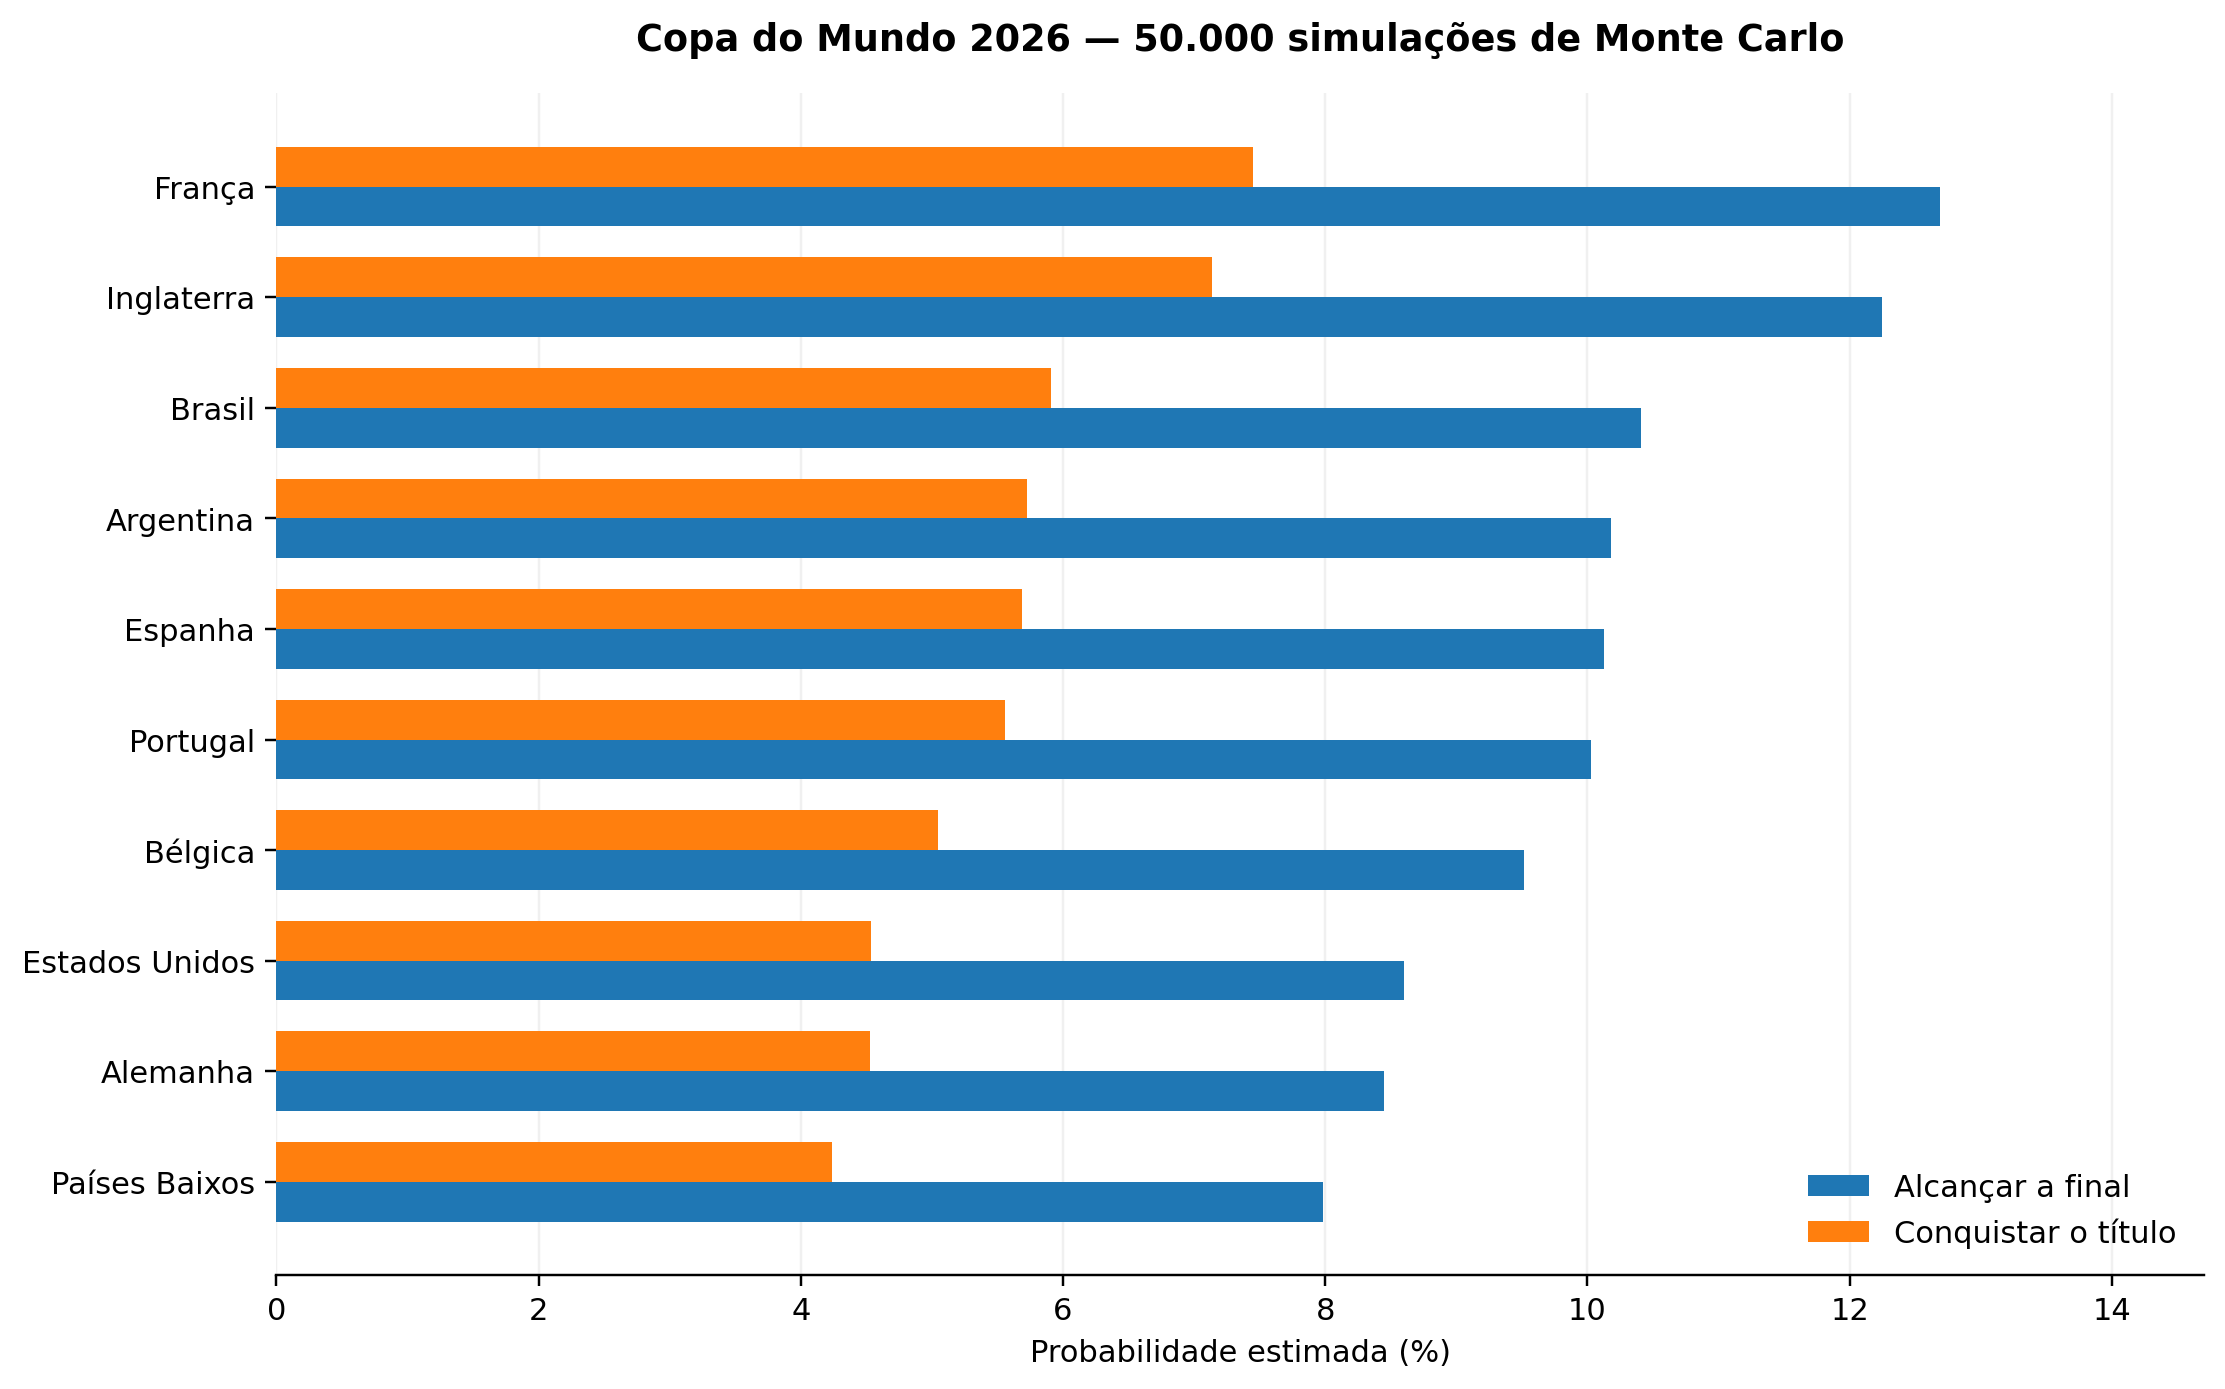
\includegraphics[width=0.96\textwidth]{figura_probabilidades_copa_2026.png}
 \caption{Probabilidades estimadas de alcançar a final e conquistar o título entre as dez principais favoritas do modelo. Fonte: simulações computacionais dos autores.}
 \label{fig:prob_copa}
\end{figure}

A França apresentou a maior probabilidade de título (7,45\%), seguida por Inglaterra (7,13\%) e Brasil (5,91\%). Apesar das diferenças na força estimada dos elencos, as probabilidades de título permaneceram distribuídas por várias equipes, refletindo a composição da incerteza ao longo de sete partidas possíveis em um torneio com 48 seleções. Entre os 1.600.000 confrontos eliminatórios amostrados nas 50.000 réplicas, 24,89\% demandaram prorrogação e 12,10\% chegaram à disputa de pênaltis. São frequências geradas pelo modelo, não taxas medidas nos jogos realizados.

Em cenários de sensibilidade, foram avaliados tanto o desempate direto por pênaltis após os 90 minutos quanto a inclusão de um sexto meio-campista, como no código inicial. Os resultados completos dessas execuções são disponibilizados nos arquivos suplementares. Os efeitos devem ser analisados separadamente da variação decorrente da amostragem aleatória e da ausência de calibração empírica dos pesos e das probabilidades de pênaltis.

A interpretação das probabilidades como prognósticos anteriores ao torneio depende ainda da confirmação da data de coleta dos atributos do \textit{Football Manager} e dos rankings utilizados, para excluir a possibilidade de vazamento temporal de informações. Este experimento deve ser descrito, até essa verificação, como uma simulação retrospectiva não condicionada aos placares reais.

\subsection{Validação no 1.º Turno do Campeonato Brasileiro Série A (Pontos Corridos)}

Diferentemente do torneio curto de seleções, a validação no Campeonato Brasileiro Série A submeteu o modelo à volatilidade de uma liga contínua de longa duração. A avaliação cobriu 189 partidas do 1.º Turno, aplicando a pipeline de Força Híbrida (50\% $CA^3$ FM26 + 50\% Tabela Real), Fator de Fase e a matriz de correção de Dixon-Coles ($\rho = -0{,}13$) \cite{dixon1997}.

O modelo alcançou uma \textbf{acurácia nominal de 47,2\%} na indicação do resultado mais provável e um \textbf{\textit{Brier Score} de $BS = 0{,}6334$} sob a correção de Dixon-Coles (frente a $BS = 0{,}6346$ na distribuição de Poisson pura, representando uma melhora marginal de 0,2\%).

Para contextualizar o \textit{Brier Score} em um cenário tridirecional (Vitória Mandante, Empate, Vitória Visitante), o limiar de aleatoriedade para palpites uniformes de probabilidade equiprovável ($p = 1/3$) é dado por $BS_{\text{aleatório}} = 2/3 \approx 0{,}6667$. O score obtido de $0{,}6334$ supera a linha de base aleatória em aproximadamente 5\%. Ademais, a acurácia nominal de 47,2\% situa-se em um patamar competitivo frente a modelos preditivos da literatura especializada, cujos índices para ligas de futebol variam habitualmente entre 50\% e 55\% devido à elevada frequência de empates e à instabilidade de resultados característica do futebol brasileiro.

O fator primário para o desvio do \textit{Brier Score} em relação ao limiar ideal teórico reside na ocorrência de empates. A distribuição de Poisson independente subestima estruturalmente os placares de igualdade; embora a correção de Dixon-Coles tenha mitigado essa limitação nos placares baixos ($0\text{--}0, 1\text{--}0, 0\text{--}1, 1\text{--}1$), a variância intrínseca dos pontos corridos impõe um desafio contínuo para a calibração probabilística em tempo real.

\subsection{Análise Comparativa e Discussão Metodológica}

A comparação entre as duas aplicações evidencia o impacto da estrutura do torneio na previsibilidade estocástica:
\begin{enumerate}
	\item \textbf{Copa do Mundo (planilha: 64,4\% de acurácia; $BS=0{,}5427$):} A avaliação original reuniu 104 placares, ressalvando-se a mistura entre resultados dos 90 minutos e da prorrogação em jogos eliminatórios. A extensão com 50.000 torneios permitiu estimar, adicionalmente, as probabilidades condicionadas à trajetória competitiva, incluindo pênaltis e classificação por fase;
	\item \textbf{Série A do Brasileirão (47,2\% de Acurácia; $BS = 0{,}6334$):} A alta competitividade do campeonato nacional, somada ao efeito de 38 rodadas e à elevada taxa de empates, elevou o ruído estatístico. Contudo, a inclusão do Fator de Fase e da Força Híbrida impediu a regressão excessiva à média, gerando projeções de pontuação final alinhadas com as faixas históricas do futebol brasileiro (campeão na faixa de 73--74 pontos).
\end{enumerate}

Em ambos os casos, a metodologia superou suas respectivas linhas de base aleatórias, comprovando a utilidade dos dados extraídos de simuladores esportivos como base secundária para a modelagem estocástica do futebol real.

\section{Considerações Finais e Perspectivas Futuras}

Os resultados obtidos neste estudo, desenvolvido no âmbito de uma iniciação científica, demonstram que a simulação de Monte Carlo (MC), acoplada à distribuição de Poisson e alimentada por metadados do \textit{Football Manager 2026} \cite{fm2026}, constitui uma estrutura computacional estocástica robusta e interpretável para a modelagem preditiva no futebol. A eficácia do arcabouço esteve alicerçada na formulação dinâmica e adaptativa do parâmetro $\lambda$ (gols esperados), capaz de ajustar-se à granularidade dos dados disponíveis em dois formatos competitivos distintos: a abordagem de razão proporcional baseada em microatributos de atletas para a Copa do Mundo de 2026, agora acompanhada de simulações integradas de classificação de grupos e mata-mata, e a abordagem de Força Híbrida acoplada ao Fator de Fase para a Série A do Campeonato Brasileiro.

\subsection{Síntese dos Resultados e Limitações do Estudo}

A validação empírica realizada sobre uma amostra abrangente de 293 partidas (104 da Copa do Mundo e 189 da Série A) superou as linhas de base aleatórias em ambos os cenários, atingindo uma acurácia preditiva de 64,4\% ($BS = 0{,}5427$) no torneio de seleções e de 47,2\% ($BS = 0{,}6334$) na liga nacional de pontos corridos. Na Copa do Mundo, a correção dos identificadores de países e a simulação integrada do torneio permitiram identificar e explorar limitações da abordagem heurística sem alterar a lógica central de Poisson. A interpretação da acurácia retrospectiva global de 104 partidas permanece condicionada à revisão dos placares referentes aos 90 minutos nas fases eliminatórias. A comparação com a Série A também requer atenção à diferença entre as estruturas competitivas e à calibração dos respectivos modelos.

A despeito dos avanços alcançados, o modelo apresenta limitações metodológicas bem delimitadas:
\begin{enumerate}
	\item \textbf{Subestimação Estrutural de Empates:} A distribuição de Poisson independente tende a subestimar a ocorrência de placares iguais. Embora a implementação da correção de Dixon-Coles ($\rho = -0{,}13$) tenha produzido uma melhora marginal no $BS$ ($0{,}2\%$), a incerteza associada a jogos parelhos permanece um desafio para modelos puramente estocásticos;
	\item \textbf{Estatismo das Variáveis de Entrada:} As simulações dependem de métricas pré-jogo do \textit{Football Manager}, omitindo eventos estocásticos dinâmicos e imponderáveis no decorrer das partidas, como expulsões precoces, lesões de atletas-chave, condições meteorológicas adversas e decisões de arbitragem;
	\item \textbf{Parametrização Heurística Manual:} A calibração dos pesos e dos limiares de truncamento ($\mathrm{clip}$) foi conduzida manualmente pelos pesquisadores, o que garante interpretabilidade ao modelo, mas limita a capacidade de aprendizado automático frente a novos padrões de dados.
 \item \textbf{Cobertura e temporalidade das bases da Copa:} A distribuição de posições de jogadores não permite completar exatamente 16 atletas em cinco seleções; alguns nomes geográficos estavam truncados; e não foram fornecidos cartões para reproduzir todos os critérios oficiais de desempate. Também são necessárias as datas de extração dos atributos para avaliar o risco de vazamento temporal e a separação dos gols no tempo regulamentar e na prorrogação para a validação das partidas eliminatórias.
\end{enumerate}

\subsection{Trabalhos Futuros e Aprendizado de Máquina}

Como desdobramento natural desta iniciação científica e escopo principal para o Trabalho de Conclusão de Curso (TCC) do discente, a pesquisa evoluirá da modelagem estocástica heurística para algoritmos de Aprendizado de Máquina orientados a dados. O próximo estágio investigativo focará em um estudo comparativo direto entre três arquiteturas preditivas:
\begin{enumerate}
	\item O modelo estocástico de Monte Carlo (MC) parametrizado nesta etapa;
	\item Redes Neurais Artificiais (RNA) do tipo \textit{Feedforward} Multicamadas (PMC), compostas por uma camada de entrada com 20 variáveis de desempenho técnico-tático, camadas ocultas com 128, 64 e 32 neurônios (ativação ReLU) e uma camada de saída \textit{Softmax} para probabilidades de vitória do mandante, empate e vitória do visitante;
	\item Regressão Linear Múltipla, atuando como \textit{baseline} estatístico paramétrico.
	\end{enumerate}
		
		O treinamento e a validação dos modelos utilizarão técnicas de validação cruzada para mitigar o risco de \textit{overfitting}, avaliando o desempenho por meio do \textit{Brier Score}, acurácia nominal e curvas de calibração probabilística. Além disso, planeja-se a transição dos dados sintéticos do \textit{Football Manager} para indicadores do futebol real, incorporando métricas do mercado profissional, como o Valor de Mercado dos elencos (\textit{Transfermarkt}) e o sistema \textit{Elo Rating}.
		
		Este trabalho estabelece um alicerce metodológico consistente para a análise preditiva esportiva, comprovando a viabilidade de simuladores virtuais como fontes legítimas de dados e delimitando as fronteiras entre a imprevisibilidade intrínseca do futebol e a precisão alcançável por métodos estocásticos e de inteligência artificial.

\bibliographystyle{plainurl}
\bibliography{biblioteca,referencias_novas}

\end{document}